%----------------------------------------------------------------------------------------
%	PACKAGES AND THEMES
%----------------------------------------------------------------------------------------
\documentclass[aspectratio=169,xcolor=dvipsnames]{beamer}
\usetheme{SimplePlusAIC}
\usepackage{xcolor}
\usepackage{hyperref}
\usepackage{graphicx} % Allows including images
\usepackage{booktabs} % Allows the use of \toprule, \midrule and  \bottomrule in tables
\usepackage{svg} %allows using svg figures
\usepackage{tikz}
\usepackage{makecell}
\newcommand*{\defeq}{\stackrel{\text{def}}{=}}
\usefonttheme[onlymath]{serif}
\usepackage{mwe,tikz}\usepackage[percent]{overpic}
\usepackage{animate}

%Select the Epilogue font (requires luaLatex or XeLaTex compilers)
\usepackage{fontspec}
\setsansfont{Epilogue}[
    Path=./epilogueFont/,
    Scale=0.9,
    Extension = .ttf,
    UprightFont=*-Regular,
    BoldFont=*-Bold,
    ItalicFont=*-Italic,
    BoldItalicFont=*-BoldItalic
    ]
\newcommand{\vect}[1]{\mathbf{#1}}
%----------------------------------------------------------------------------------------
%	TITLE PAGE
%----------------------------------------------------------------------------------------

\title[short title]{Optimální tvar stěn idealizovaného\\ kavopulmonálního spojení} % The short title appears at the bottom of every slide, the full title is only on the title page
\subtitle{Diplomová práce}

\author[Surname]{Jan Bureš\textmd{, Radek Fučík, Radomír Chabiniok}}
\institute[KM FJFI 2024]{Katedra matematiky \newline Fakulta jaderná a fyzikálně inženýrská\newline České vysoké učení technické v Praze}
% Your institution as it will appear on the bottom of every slide, maybe shorthand to save space


\date{11. prosince 2024} % Date, can be changed to a custom date
%----------------------------------------------------------------------------------------
%	PRESENTATION SLIDES
%----------------------------------------------------------------------------------------

\begin{document}

\begin{frame}[plain, noframenumbering]
    % Print the title page as the first slide
    \vspace{-21mm}
    \titlepage
\end{frame}

\begin{frame}[plain, noframenumbering]{Přehled}
    % Throughout your presentation, if you choose to use \section{} and \subsection{} commands, these will automatically be printed on this slide as an overview of your presentation
    \tableofcontents
\end{frame}

%------------------------------------------------
\section{Motivace}
%------------------------------------------------

\begin{frame}{Motivační úloha}
	\begin{columns}[T] % align columns
		\begin{column}{.63\textwidth}
			\begin{figure}
				\includegraphics[width=0.9\linewidth]{Images/srdce_zoom_cz.pdf}
			\end{figure}
		\end{column}%
		\hfill%
		\begin{column}{.37\textwidth}
			\vspace{0pt}
			\textbf{Optimalizační úloha:}\\
			\vspace{6pt}
			Nalézt minimum
			\begin{equation*}
				\min _{\vect{x} \in \mathbb{X} } f \ (\vect{x}),
			\end{equation*}
			kde $ f \ (\vect{x}) $ je účelová funkce.\\ \pause
			\vspace{11pt}
			\textbf{Charakterizace:}\\[2pt]
			\begin{itemize}
				\item nelineární
				\item s vazbami
			\end{itemize}
		\end{column}%
	\end{columns}
\end{frame}

%------------------------------------------------
\section{Optimalizační rámec}
%------------------------------------------------
\begin{frame}{Rámec}
	
	\begin{figure}
		\includegraphics[width=0.95\linewidth, trim={0 -0.1cm 0 0}, clip]{Images/framework-cz.pdf}
	\end{figure}
\end{frame}
%------------------------------------------------
\begin{frame}{Rámec}
	\addtocounter{framenumber}{-1}
	\begin{figure}
		\includegraphics[width=0.95\linewidth, trim={0 -0.1cm 0 0}, clip]{Images/framework-cz-1.pdf}
	\end{figure}
\end{frame}
%------------------------------------------------
\begin{frame}{Mřížková Boltzmannova metoda}
	\begin{columns}[T] % align columns
		\begin{column}{.45\textwidth}
			\textbf{LBM:} - KM FJFI\\
			\begin{itemize}
				\item rychlostní model D3Q27, CuLBM
			\end{itemize}
		\begin{eqnarray*}
			\rho &=& \sum_{k=1}^{27} f_{k}\\
			\rho \vect{u} &=& \sum_{k=1}^{27} f_{k} \boldsymbol{\xi}_{k} + \dfrac{\Delta t}{2} \rho \boldsymbol{g}
		\end{eqnarray*}
			\textbf{Okrajové a počáteční podmínky:}\\
			\begin{itemize}
				\item hranice oblasti $ \rightarrow $ symetrické OP
				\item hranice objektu $ \rightarrow $ bounce-back
				\item rovnovážná počáteční podmínka
			\end{itemize}
		\end{column}%
		\begin{column}{.5\textwidth}
			\textbf{Rovnice dynamiky tekutin:}
			\vspace{-13pt}
			\begin{center}
				$$\frac{\partial \rho}{\partial t} + \nabla \cdot (\rho \vect{u}) = 0 $$
				$$\frac{\partial (\rho \vect{u})}{\partial t} + \nabla \cdot (\rho \vect{u} \otimes \vect{u}) = \nabla \cdot \mathbf{T} + \rho \boldsymbol{g}$$
			\end{center}%
			\vspace{11pt}
			\textbf{Předpoklady:}\\[2pt]
			\begin{itemize}
				\item izotermální systém bez vnějších sil
				\item nestlačitelná newtonovská tekutina
			\end{itemize}
		\end{column}%
	\end{columns}
\end{frame}
%%------------------------------------------------
\begin{frame}{Rámec}
	\addtocounter{framenumber}{-1}
	\begin{figure}
		\includegraphics[width=0.95\linewidth, trim={0 -0.1cm 0 0}, clip]{Images/framework-cz-2.pdf}
	\end{figure}
\end{frame}
%------------------------------------------------
\begin{frame}{Generování geometrie}
	\begin{itemize}
		\item balík vytvořený pro účely parametrického generování geometrie a následné voxelizace
	\end{itemize}
	\begin{figure}
		\includegraphics[width=0.8\linewidth, trim={0 -0.1cm 0 0}, clip]{Images/meshgen.pdf}
	\end{figure}
\end{frame}
%------------------------------------------------
\begin{frame}{Generování geometrie - šablona}
	\begin{figure}
		\includegraphics[width=0.6\linewidth, trim={0 -0.1cm 0 0}, clip]{Images/meshgen-1.pdf}
	\end{figure}
\end{frame}
%------------------------------------------------
\begin{frame}{Generování geometrie - STL}
	\begin{figure}
		\includegraphics[width=0.6\linewidth, trim={0 -0.1cm 0 0}, clip]{Images/meshgen-2.pdf}
	\end{figure}
\end{frame}
%------------------------------------------------
\begin{frame}{Generování geometrie - voxelizace}
	\begin{figure}
		\includegraphics[width=0.6\linewidth, trim={0 -0.1cm 0 0}, clip]{Images/meshgen-3.pdf}
	\end{figure}
\end{frame}
%------------------------------------------------
\begin{frame}{Generování geometrie - výsledek}
	\begin{figure}
		\includegraphics[width=0.6\linewidth, trim={0 -0.1cm 0 0}, clip]{Images/meshgen-4.pdf}
	\end{figure}
\end{frame}
%------------------------------------------------
\begin{frame}{Rámec}
	\addtocounter{framenumber}{-1}
	\begin{figure}
		\includegraphics[width=0.95\linewidth, trim={0 -0.1cm 0 0}, clip]{Images/framework-cz-3.pdf}
	\end{figure}
\end{frame}

%------------------------------------------------
\begin{frame}{Optimalizace}
	\begin{itemize}
		\setlength\itemsep{1.8em}
		\item Předchozí práce (VÚ) $\Rightarrow$ bezgradientní metody
		\item Úloha s vazbami $\Rightarrow$ extrémní bariérová metoda
		\item Vyčíslení $ f \ (x \, ) $ pomocí LBM $\Rightarrow$ \alert{výpočetně i časově náročné}
		\item Algoritmy:
			 \begin{itemize}
				\item[-] Nelderova-Meadova metoda -- vlastní implementace podporující paralelizaci
				\item[-] Mesh Adaptive Direct Search (NOMAD [1])
			 \end{itemize}
	\end{itemize}
\vspace{5.5mm}
\tiny{[1] C. Audet, et al. (2022)}, \textit{Algorithm~1027: NOMAD version~4: Nonlinear optimization with the MADS algorithm.}, DOI: 10.1145/3544489\\
\end{frame}



%------------------------------------------------
\section{Výsledky}
%------------------------------------------------
\begin{frame}{Výsledky}
	\begin{itemize}
		\setlength\itemsep{1.4em}
		\item Použití balíku \texttt{meshgen}, řešení netriviálních úloh
		\item Reynoldsův rozklad:
				$$ \vect{u} \,(x, y, z, t) = \overline{\vect{u} \,(x, y, z)} + \vect{u}^\prime(x, y, z, t) $$
		\item Účelové funkce: turbulentní kinetická energie a smyková rychlost
				$$ T_{\mathrm{turb}} = \frac{1}{2} (\vect{u}^\prime(x, y, z, t) )^2, \hspace{5mm} \dot{\gamma} = \sqrt{2} || \, \mathbf{D} \, ||^{}_{F}$$
		\item Nestlačitelná newtonovská tekutina, 3D
	\end{itemize}
\end{frame}

%------------------------------------------------
\begin{frame}{1 parametr - posun IVC}
	\begin{center}	
		\includegraphics[width=0.7\linewidth, trim={0 0 0 0}, clip]{Images/3d-tcpc-schema-combined.pdf}	
	\end{center}		
\end{frame}
%------------------------------------------------
\begin{frame}{1 parametr - posun IVC}
	\begin{itemize}
		\item Posun osy IVC, ozn. $o_1$, je jediný optimalizační parametr
	\end{itemize}
	\begin{center}
		\includegraphics[width=0.55\linewidth, trim={0 0 0 36mm}, clip]{Images/model1.pdf}
	\end{center}			
\end{frame}
%%------------------------------------------------
\begin{frame}{1 parametr - účelové funkce}
	\begin{itemize}
		\item Hodnoty účelových funkcí v závislosti na posunu $o_1$ (pouze nezáporný posun)
	\end{itemize}
	\begin{columns}
		\begin{column}{.5\textwidth}
			\includegraphics[width=1\linewidth, trim={0 0 0 0}, clip]{Images/stress.pdf}			
		\end{column}
		\begin{column}{.5\textwidth}
			\includegraphics[width=1\linewidth, trim={0 0 0 0}, clip]{Images/tke.pdf}
		\end{column}
	\end{columns}
\end{frame}
%------------------------------------------------
\begin{frame}{1 parametr}
	\begin{itemize}
		\item Určení vazeb pro posun dle fyziologických požadavků $\Rightarrow$ 0 cm až 1.2 cm
	\end{itemize}
	\begin{center}
%		\vspace{-0.5cm}
		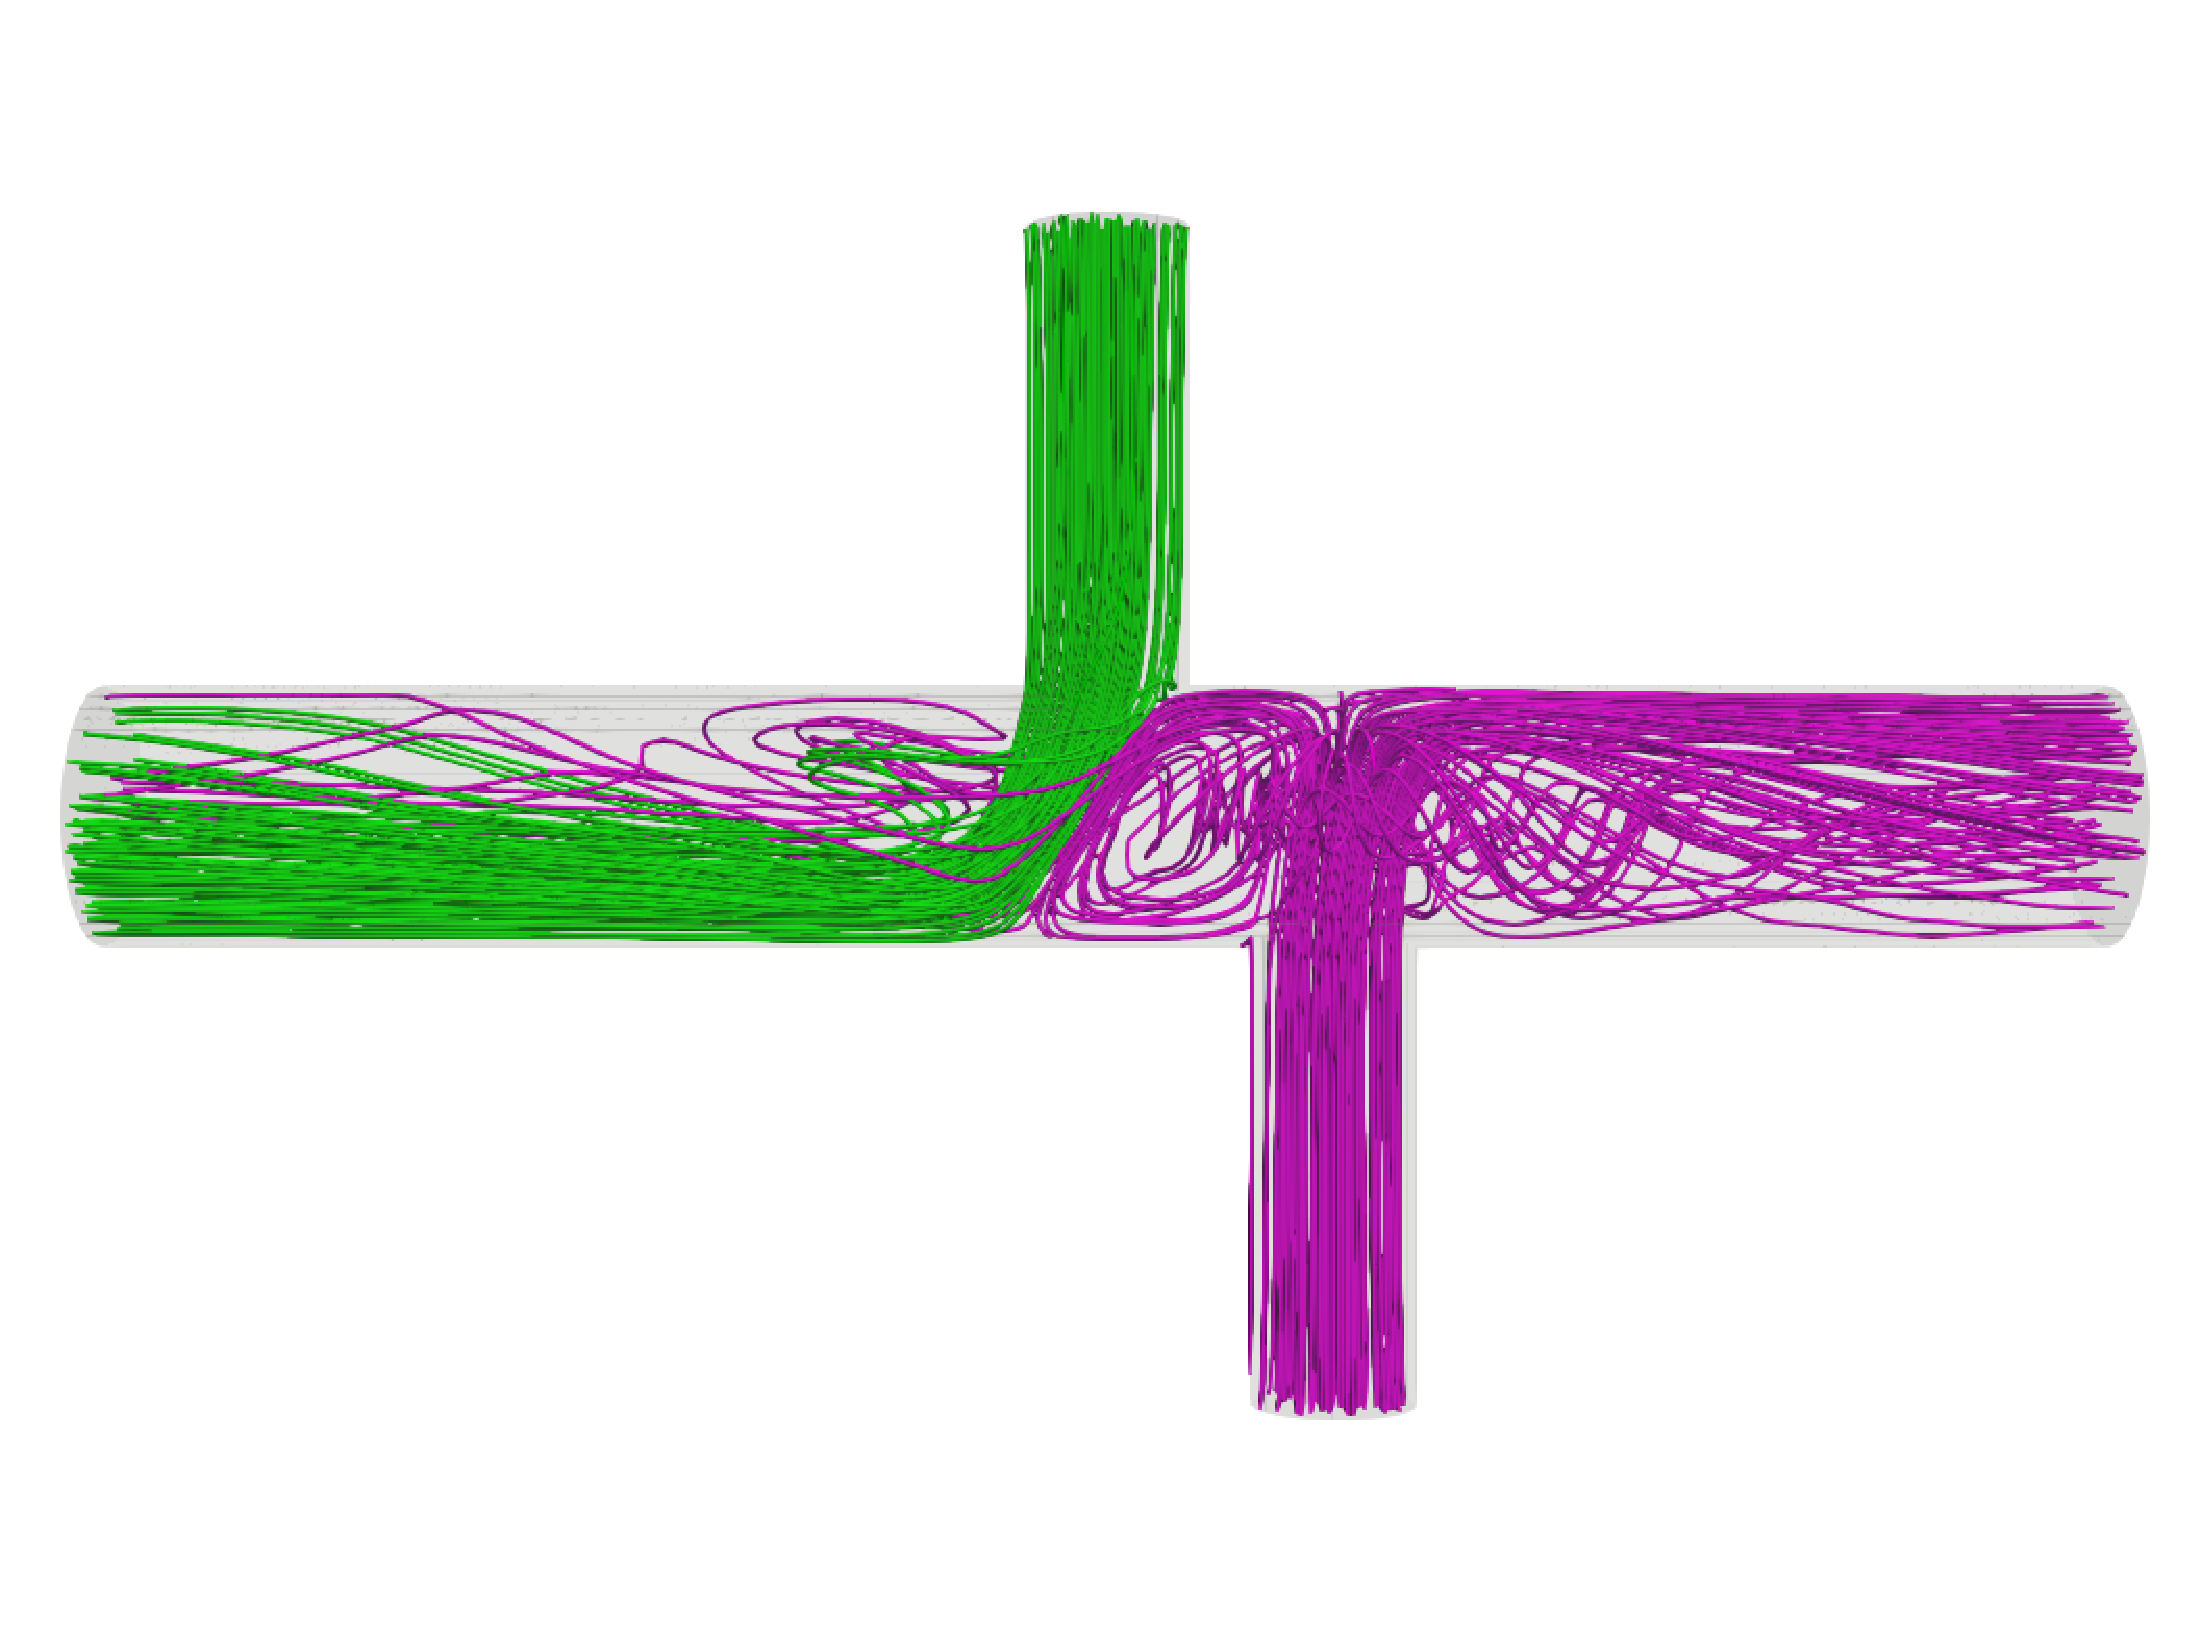
\includegraphics[width=0.55\linewidth, trim={0 0 0 0mm}, clip]{Images/IVCsplit.pdf}
		\centering
		\includegraphics[width=0.15\linewidth, trim={0 0 0 0mm}, clip]{Images/split-leg.pdf}
	\end{center}			
\end{frame}
%------------------------------------------------
\begin{frame}{1 parametr - minimalizace smykové rychlosti}
	\begin{columns}
		\begin{column}{.5\textwidth}
			\centering
			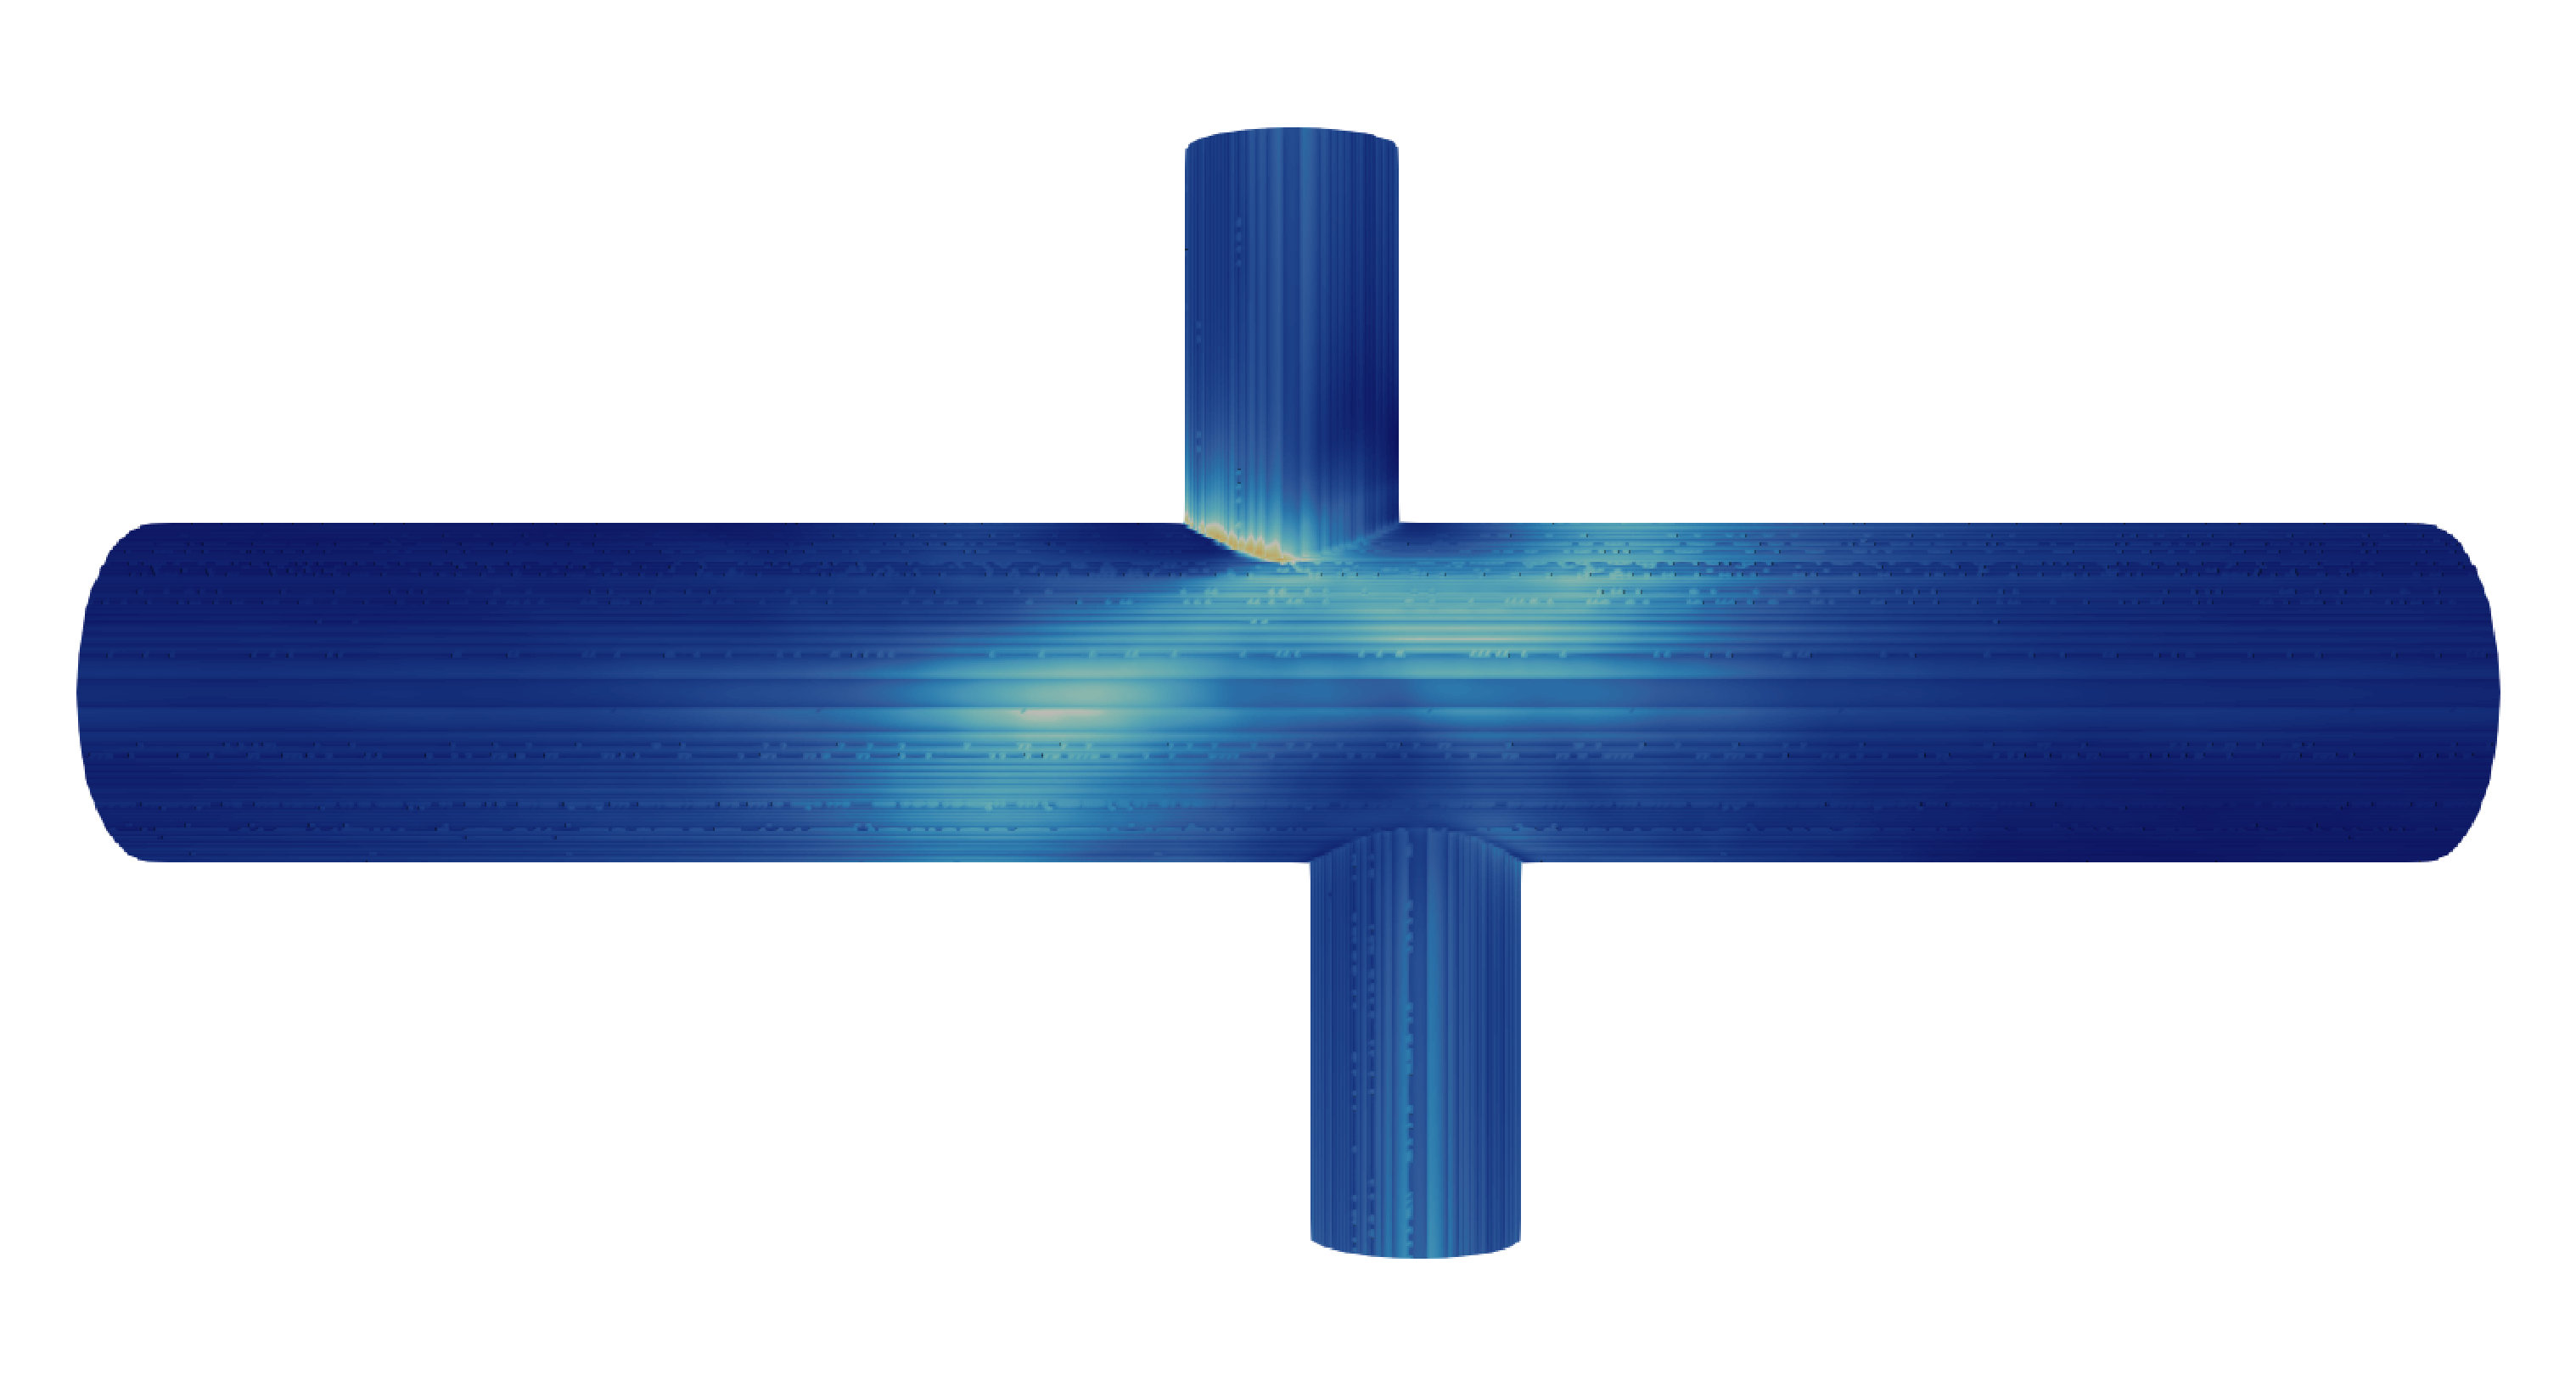
\includegraphics[width=1\linewidth, trim={0 0 0 0}, clip]{Images/08stress-side.pdf}
			\includegraphics[width=0.65\linewidth, trim={0 0 0 0}, clip]{Images/stress_leg.pdf}			
		\end{column}
		\begin{column}{.5\textwidth}
			\centering
			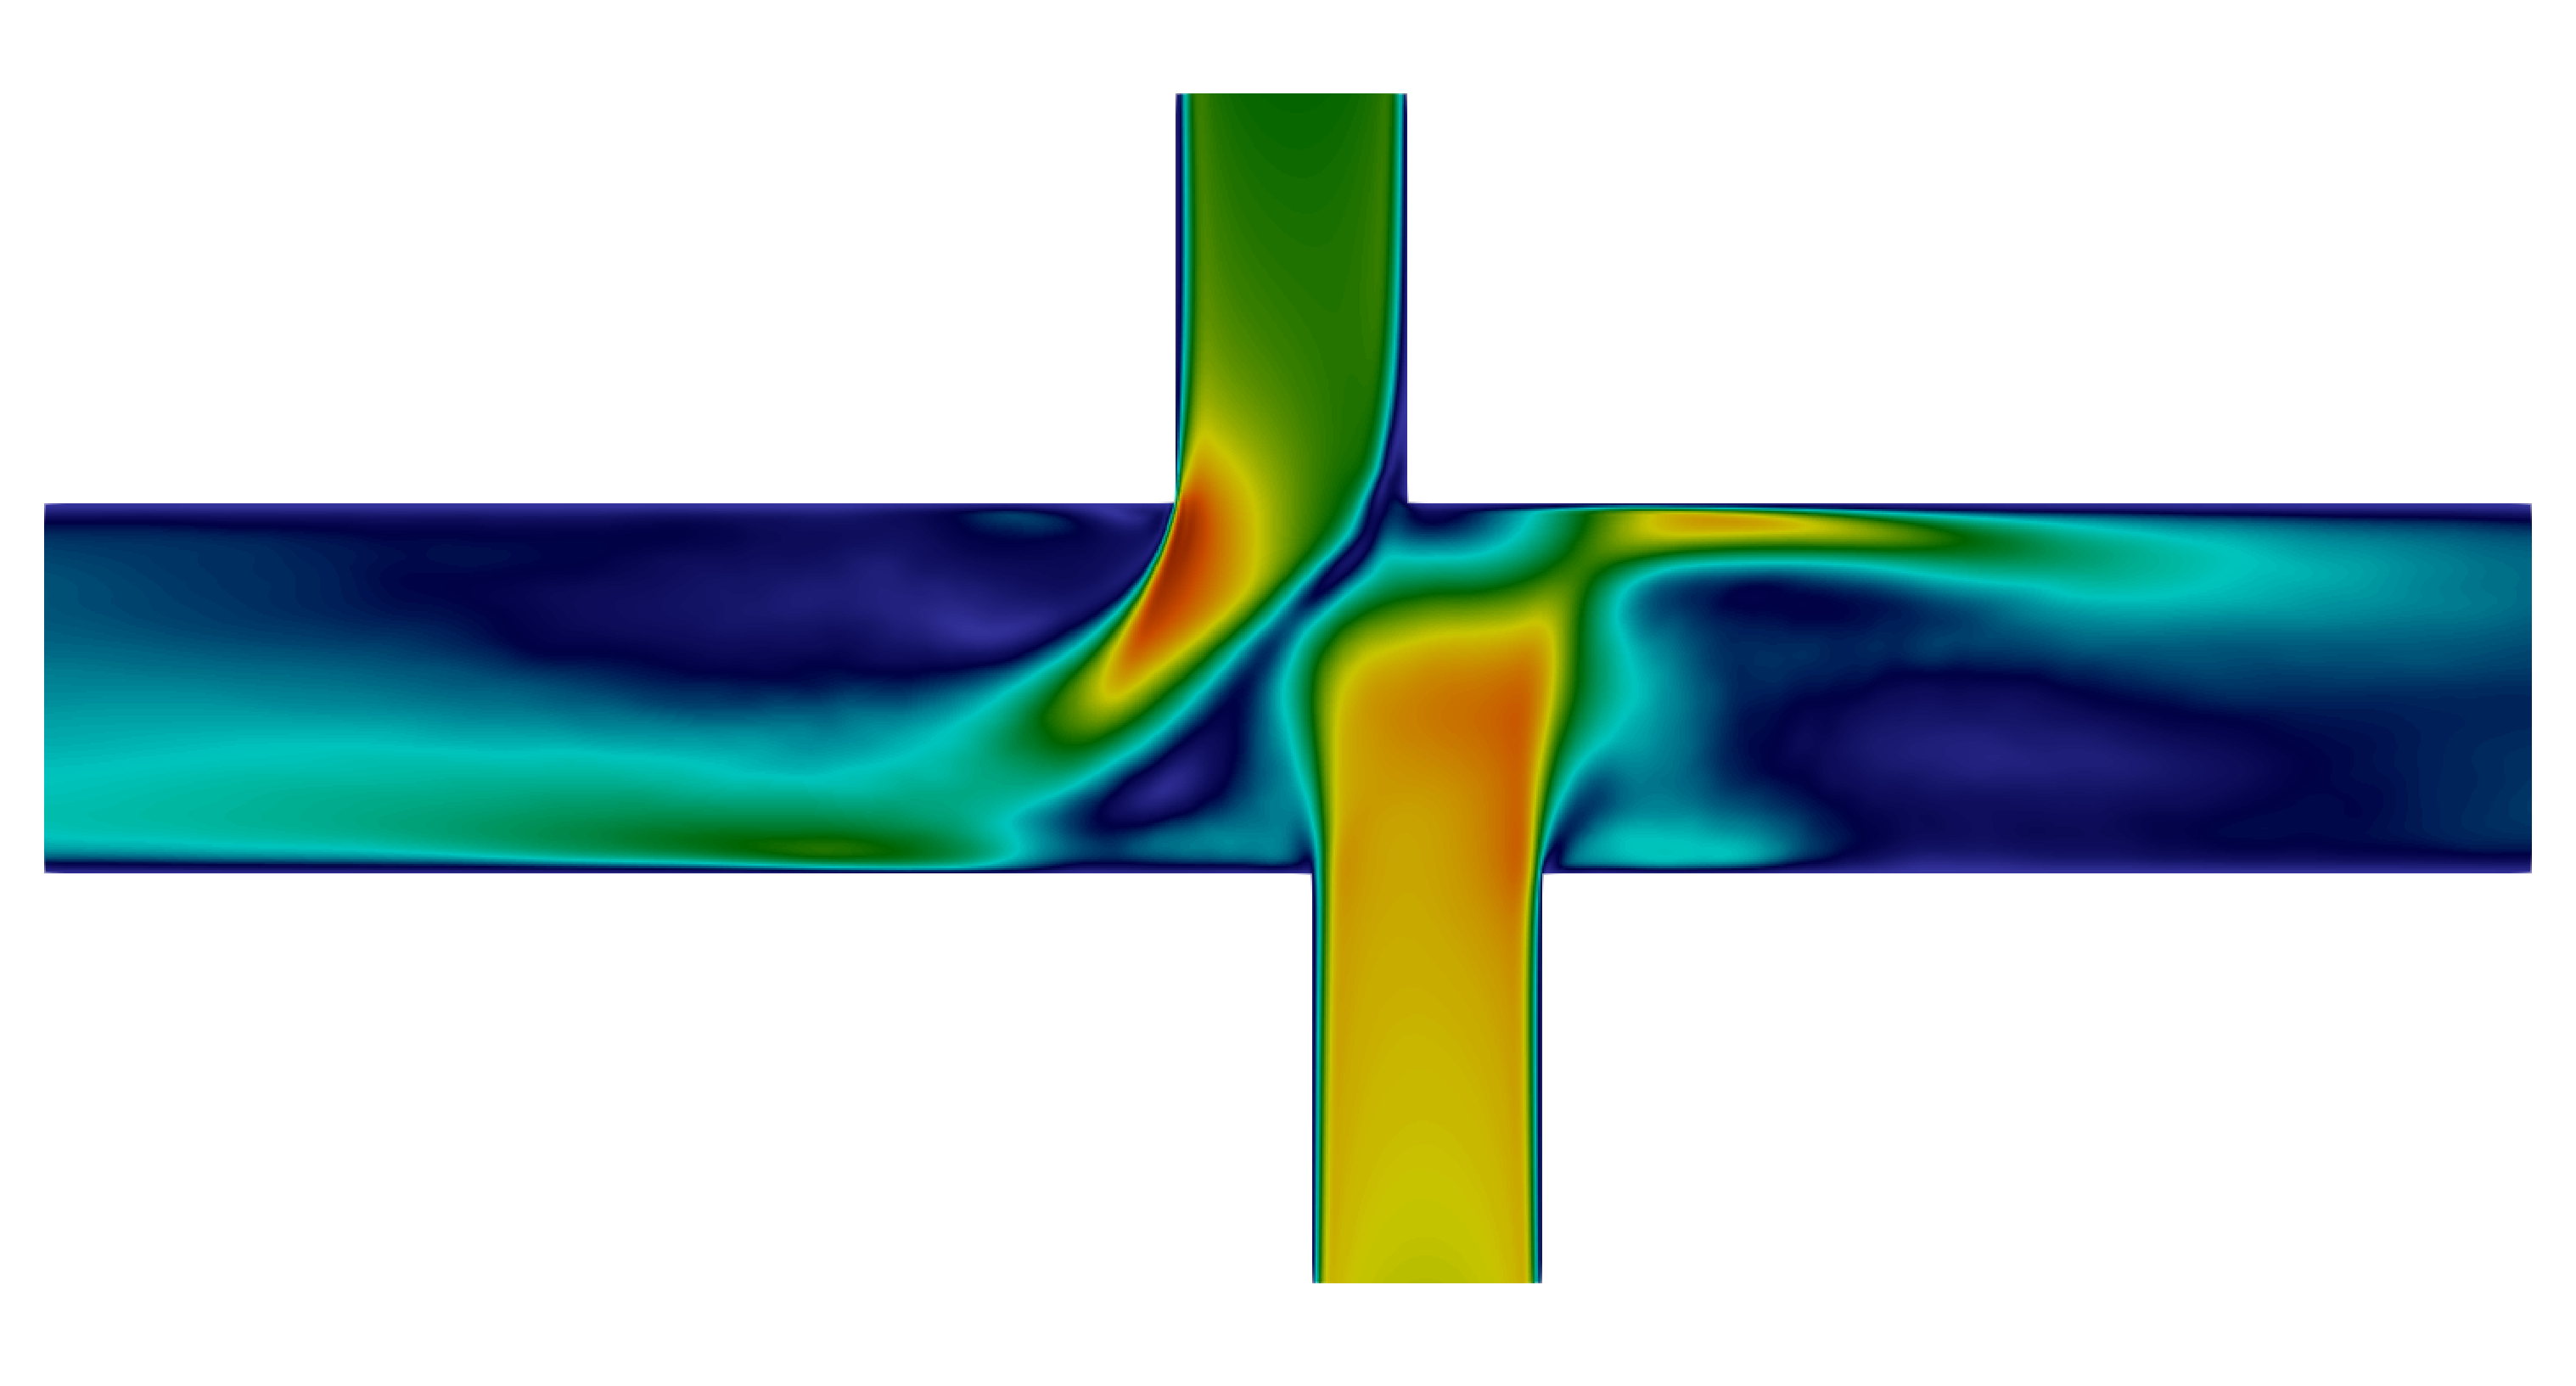
\includegraphics[width=1\linewidth, trim={0 0 0 0}, clip]{Images/08velocity-side.pdf}
			\includegraphics[width=0.65\linewidth, trim={0 0 0 0}, clip]{Images/mean_velocity_leg.pdf}
		\end{column}
	\end{columns}	
	\vspace{3mm}
	\begin{center}
		\includegraphics[width=.18\linewidth, trim={0 0 0 0}, clip]{Images/stress-mini.pdf}
	\end{center}	
\end{frame}
%------------------------------------------------
\begin{frame}{1 parametr - minimalizace smykové rychlosti}
	\begin{columns}
		\begin{column}{.5\textwidth}
			\centering
			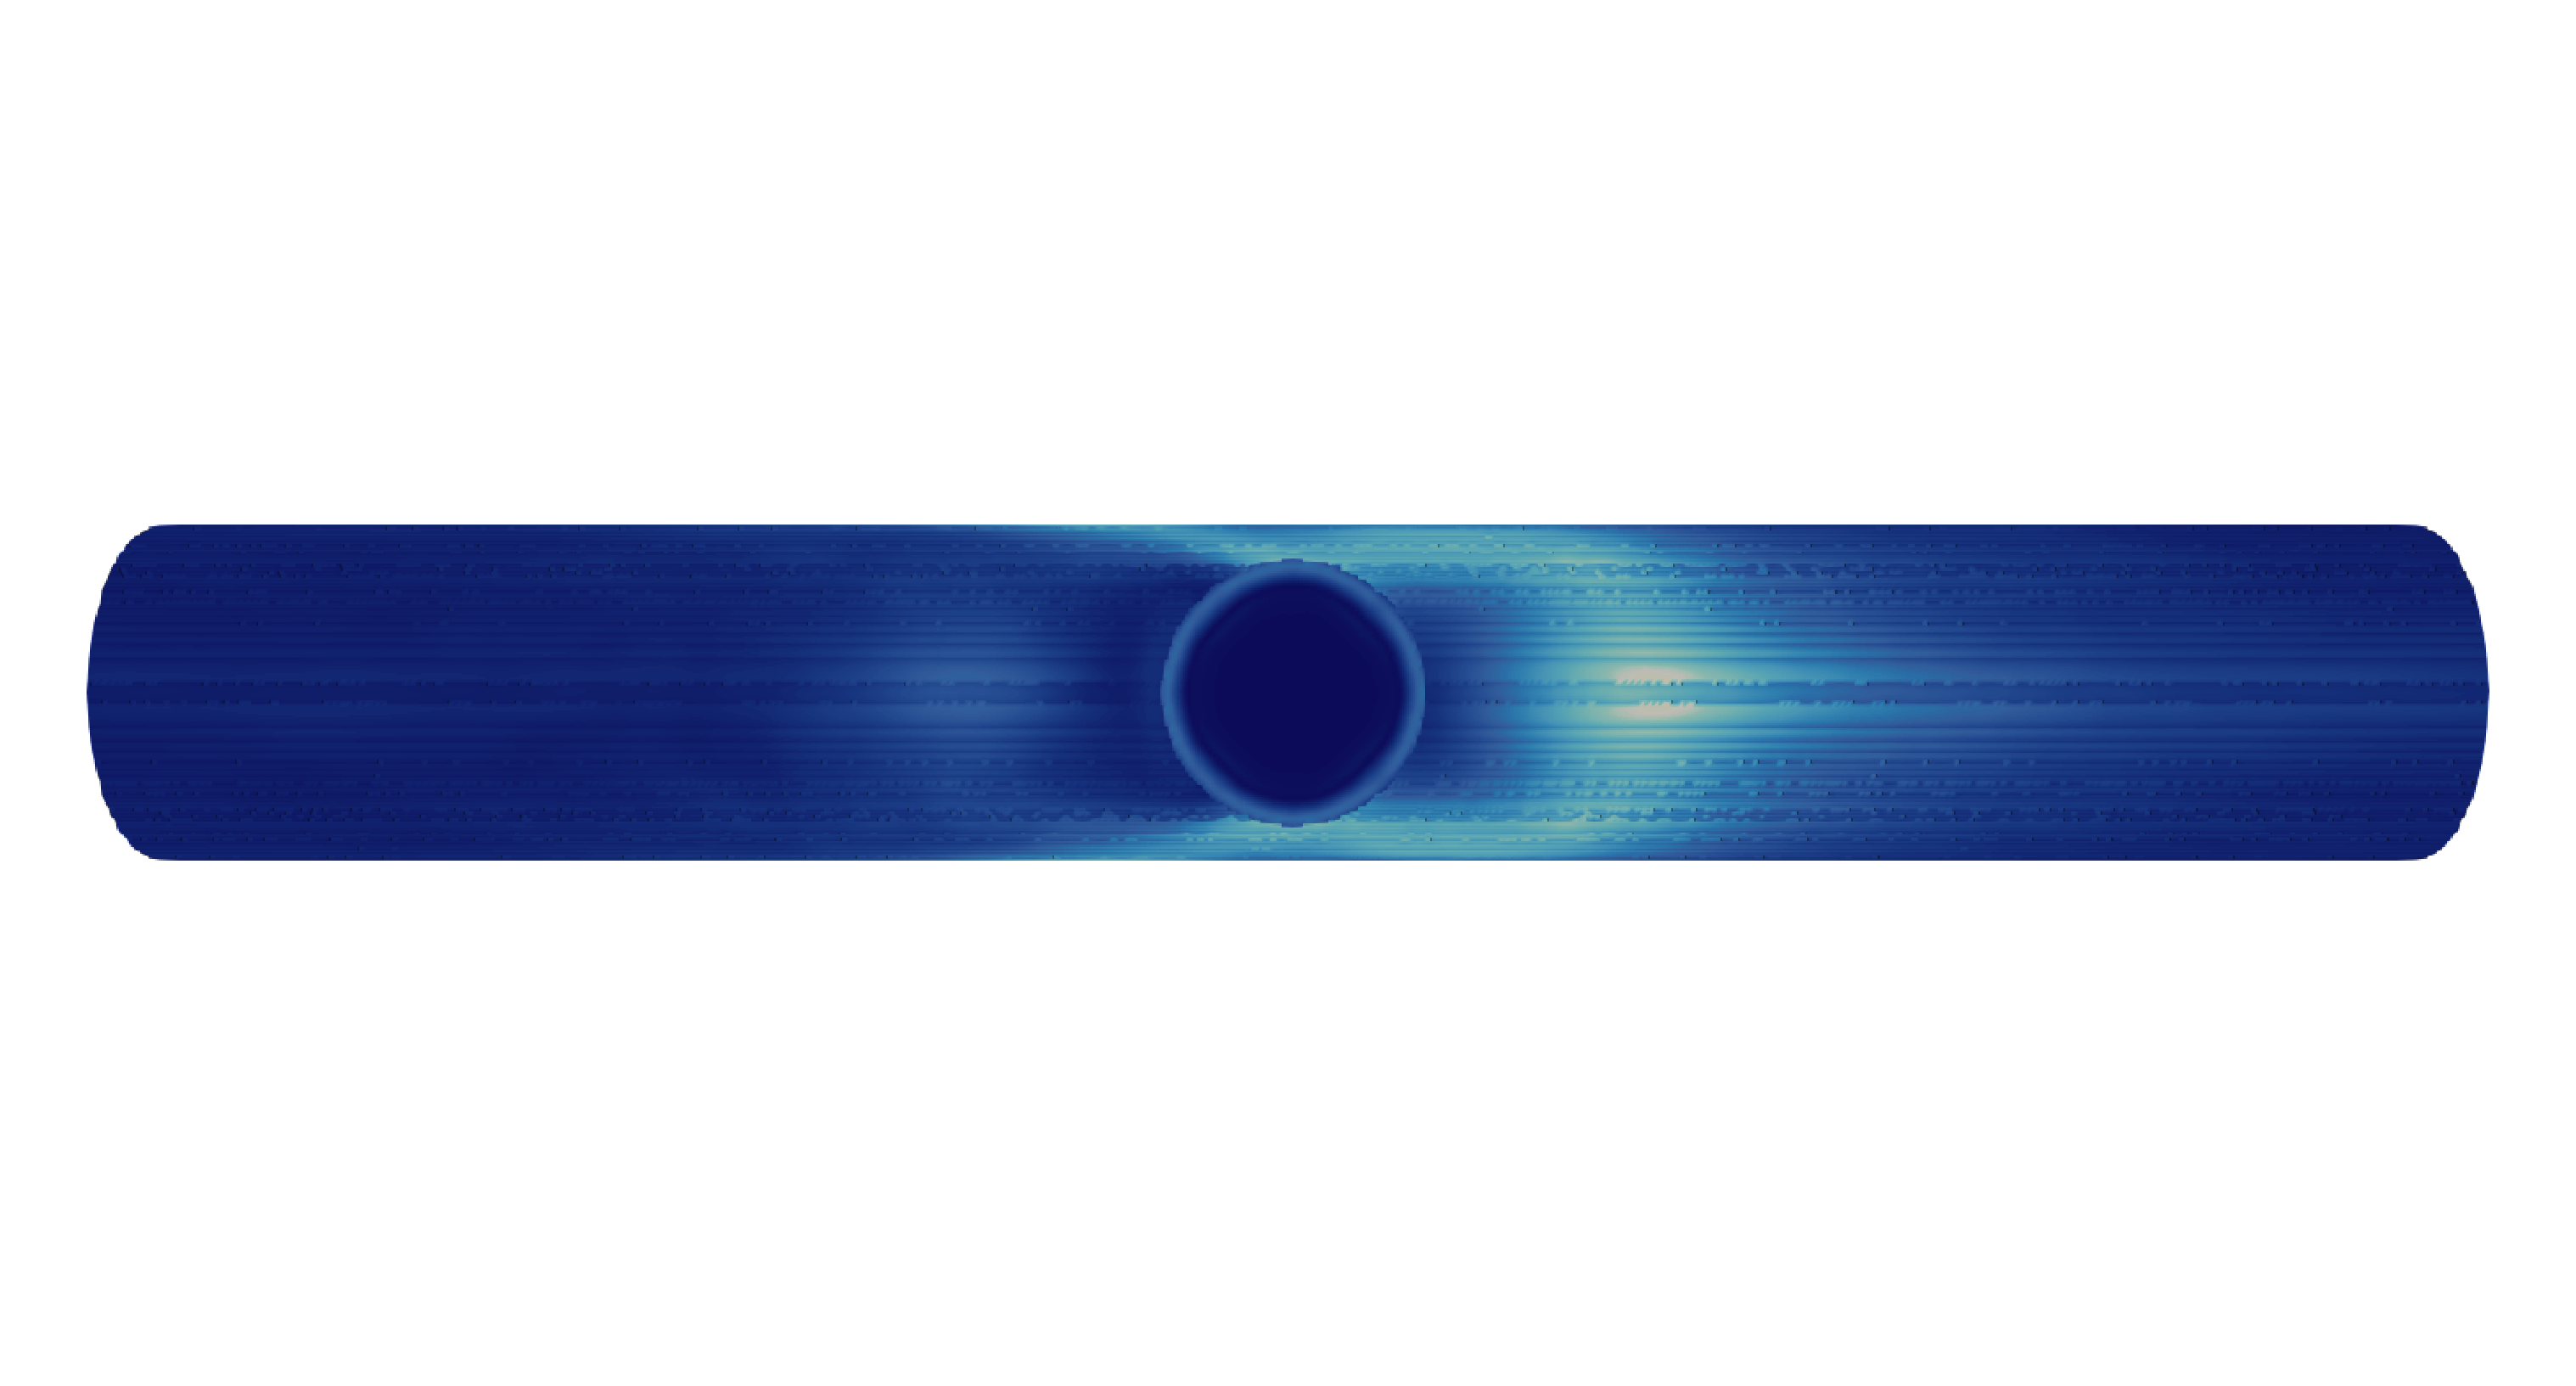
\includegraphics[width=1\linewidth, trim={0 0 0 0}, clip]{Images/08stress-top.pdf}
			\includegraphics[width=0.65\linewidth, trim={0 0 0 0}, clip]{Images/stress_leg.pdf}			
		\end{column}
		\begin{column}{.5\textwidth}
			\centering
			\includegraphics[width=1\linewidth, trim={0 0 0 0}, clip]{Images/helix.pdf}
			\includegraphics[width=0.65\linewidth, trim={0 0 0 0}, clip]{Images/mean_velocity_leg.pdf}
		\end{column}
	\end{columns}	
	\vspace{3mm}
	\begin{center}
		\includegraphics[width=.18\linewidth, trim={0 0 0 0}, clip]{Images/stress-mini.pdf}
	\end{center}	
\end{frame}
%------------------------------------------------
\begin{frame}{1 parametr - minimalizace TKE}
	\begin{columns}
		\begin{column}{.5\textwidth}
			\centering
			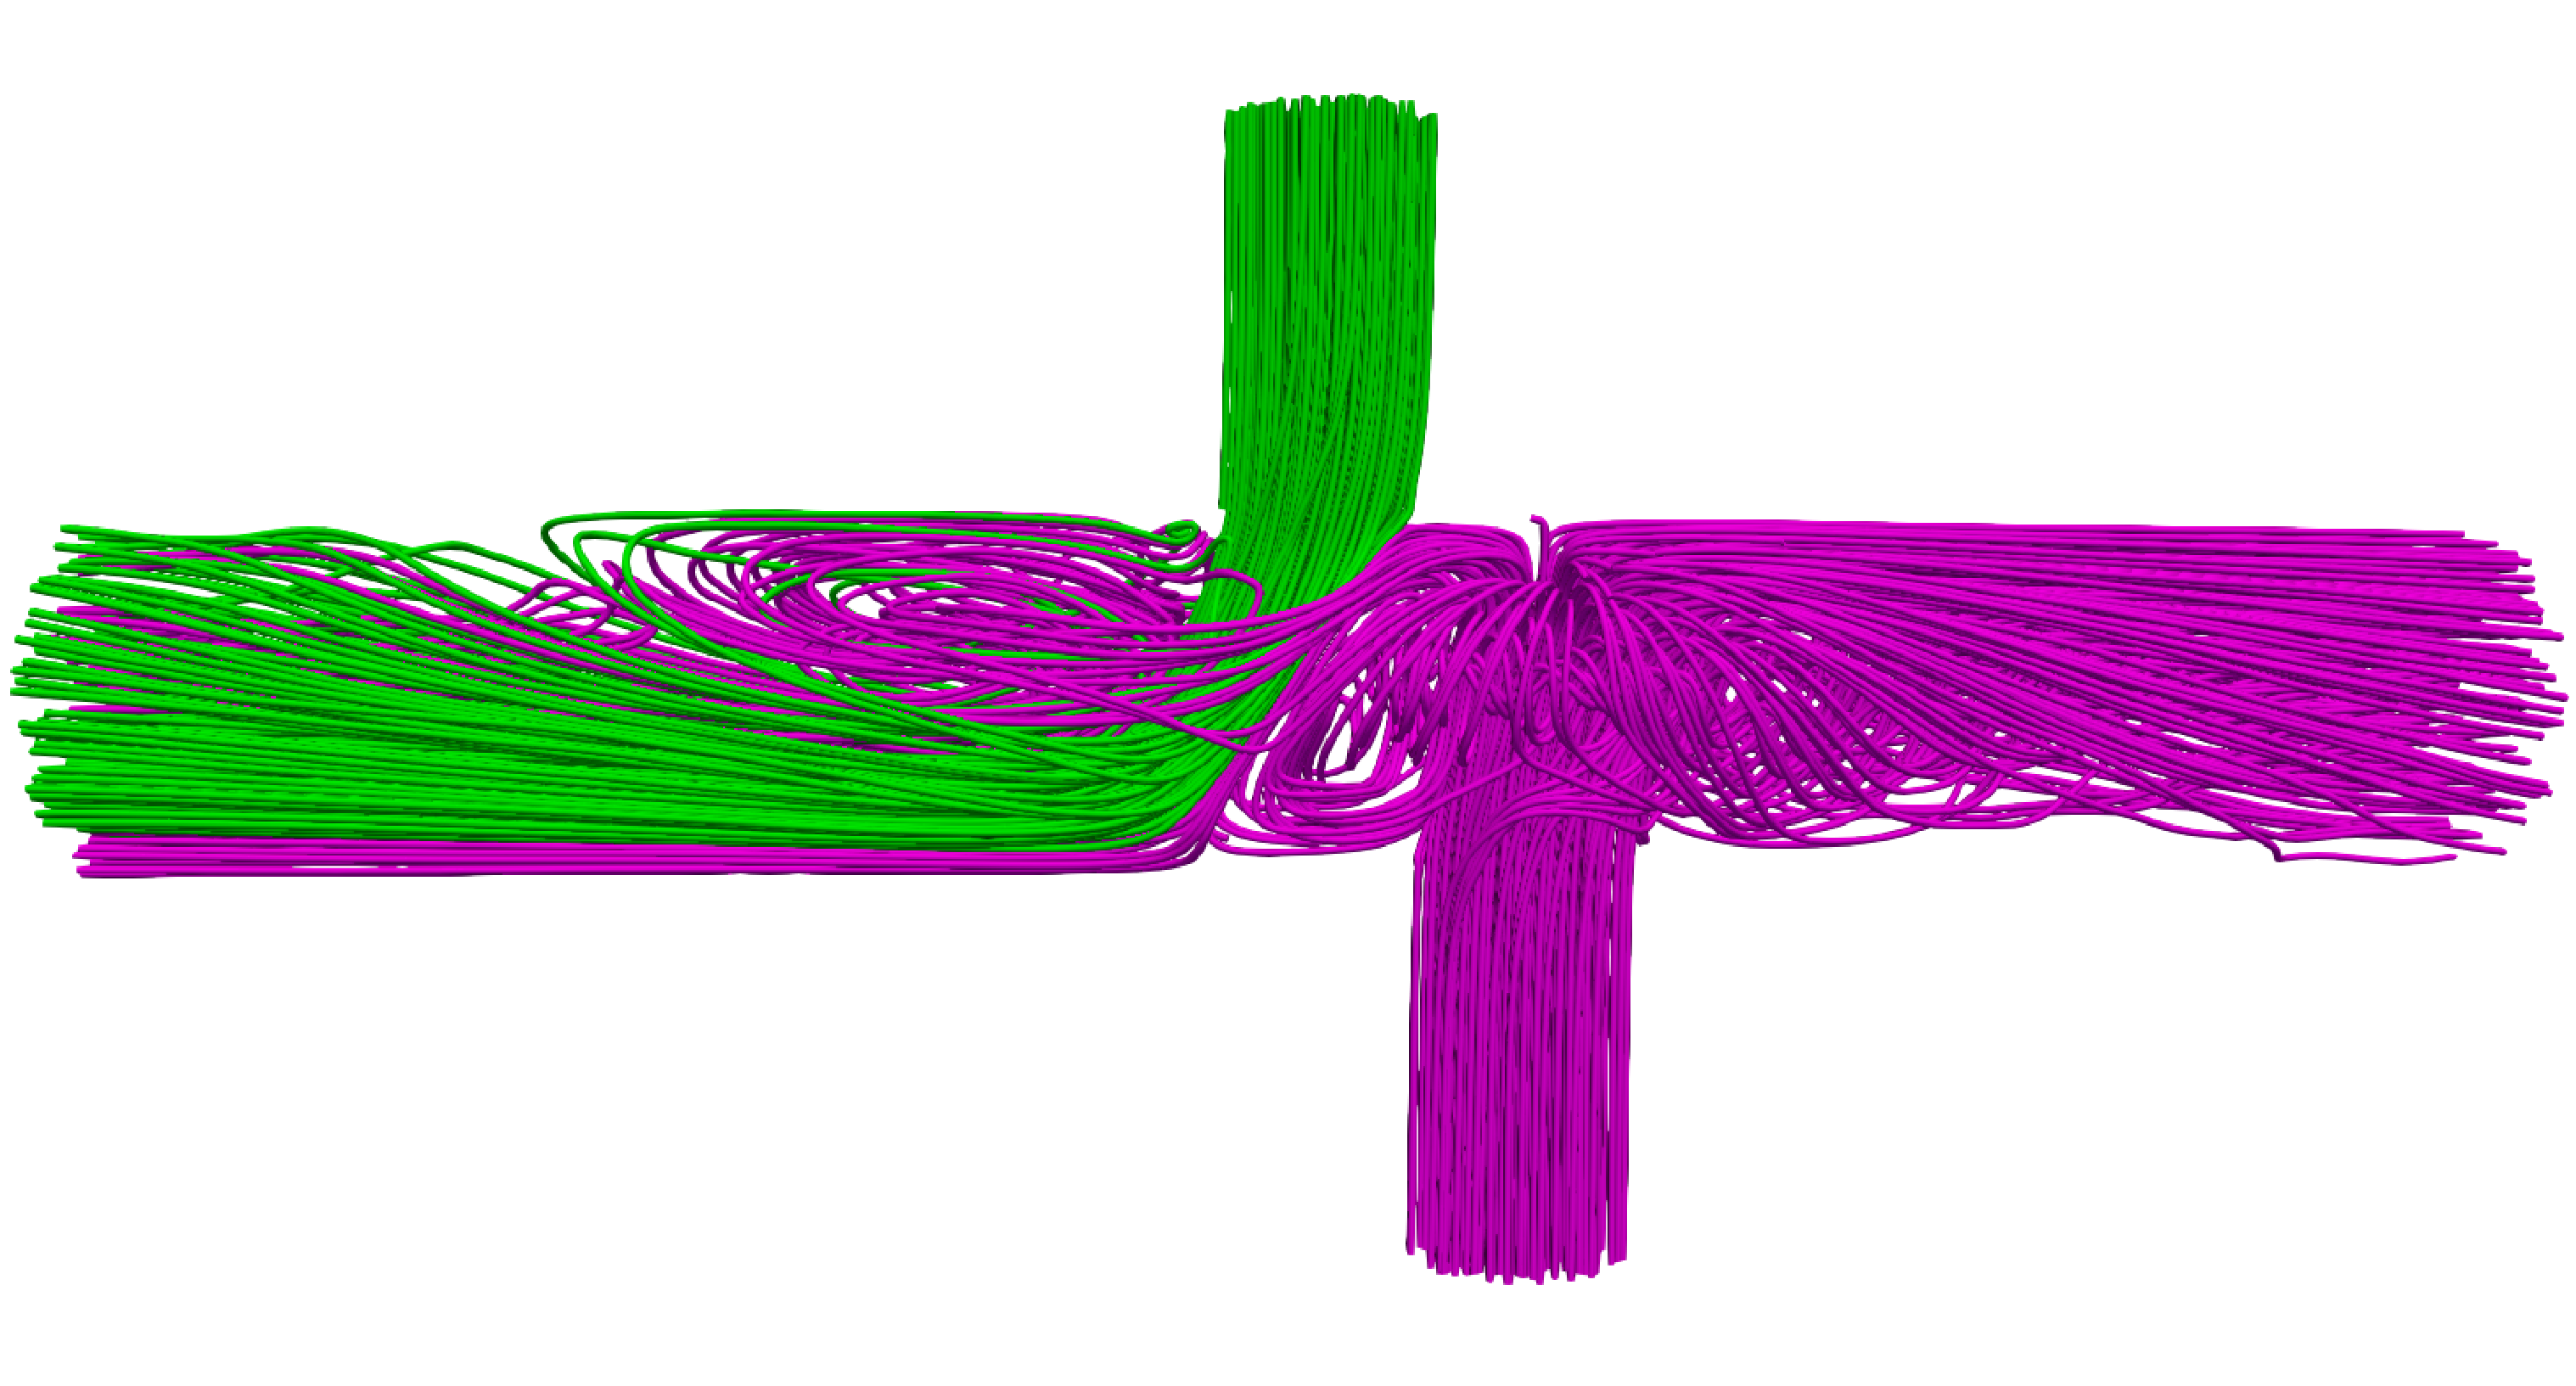
\includegraphics[width=1\linewidth, trim={0 -2mm 0 0}, clip]{Images/12IVCsplit.pdf}
			\includegraphics[width=0.33\linewidth, trim={0 0 0 0mm}, clip]{Images/split-leg.pdf}			
		\end{column}
		\begin{column}{.5\textwidth}
			\centering
			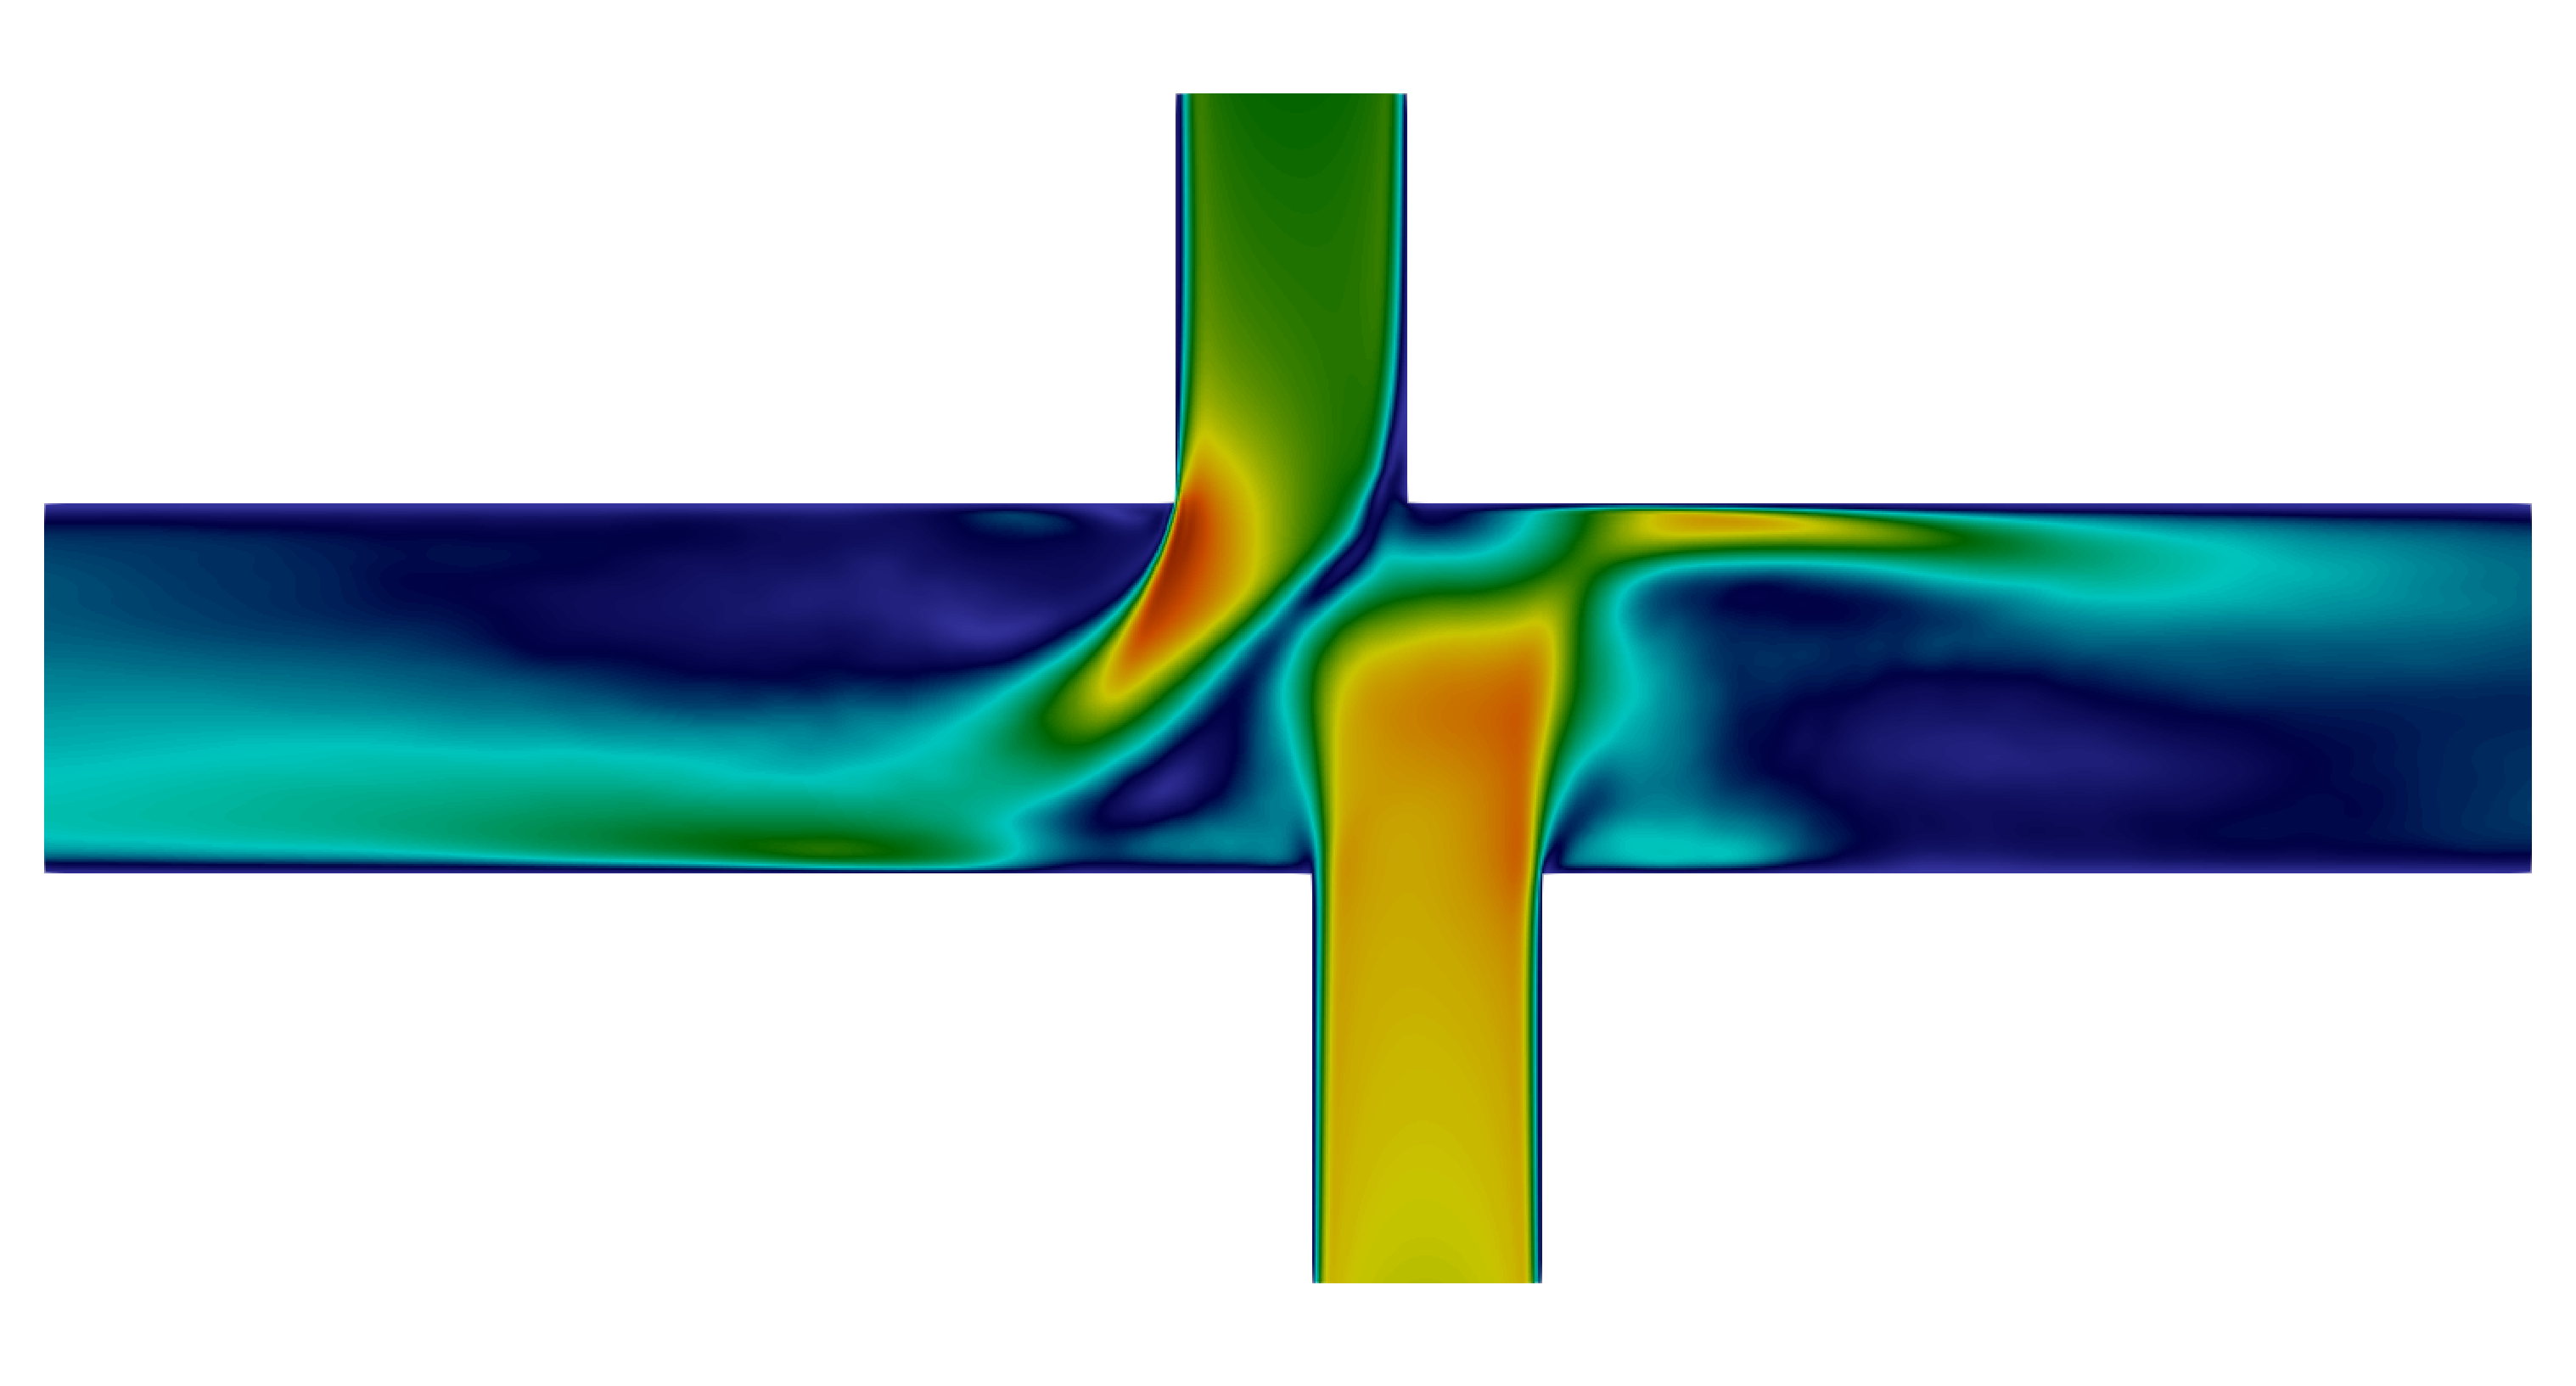
\includegraphics[width=1\linewidth, trim={0 0 0 0}, clip]{Images/08velocity-side.pdf}
			\includegraphics[width=0.65\linewidth, trim={0 0 0 0}, clip]{Images/mean_velocity_leg.pdf}
		\end{column}
	\end{columns}	
	\vspace{3mm}
	\begin{center}
		\includegraphics[width=.18\linewidth, trim={0 0 0 0}, clip]{Images/tke-mini.pdf}
	\end{center}	
\end{frame}
%%------------------------------------------------

\begin{frame}{Shrnutí}
%	\addtocounter{framenumber}{-1}
%	\setcounter{framenumber}{15}

	\begin{itemize}
		\setlength\itemsep{1.1em}
		\item Vytvořen rámec pro generování a řešení netriviálních optimalizačních úloh s pomocí LBM
		\item Navrženy parametrické modely idealizovaného TCPC
		\item Plány do budoucna: otestování komplexnějšího modelu s více parametry ¨(DP), experimenty na MRI
	\end{itemize}
	\vfill%
	\huge{\centerline{\textbf{Děkuji za pozornost!}}}
\end{frame}
%------------------------------------------------
%%\begin{frame}{Zdroje}
%%    % Beamer does not support BibTeX so references must be inserted manually as below
%%    \footnotesize{
%%    	\begin{thebibliography}{99}
%%    		\bibitem[Smith, 2012]{p1} [1] Eichler P., Fučík R., Strachota P. (2022)
%%    		\newblock Investigation of mesoscopic boundary conditions for lattice Boltzmann method
%%    		in laminar flow problems.
%%    		\newblock preprint submitted to \emph{Comput. Math. with Appl.}.
%%    	\end{thebibliography}
%%    }
%%    \footnotesize{
%%        \begin{thebibliography}{99}
%%            \bibitem[Smith, 2012]{p1} [2] Bouzidi M., Firdaouss M., Lallemand P. (2001)
%%            \newblock Momentum transfer of a Boltzmann-lattice fluid with boundaries.
%%            \newblock \emph{Physics of Fluids} 13(11), 3452–3459.
%%        \end{thebibliography}
%%    }
%%	\vspace{1cm}
%%
%%	Všechny obrázky bez citace jsou originální nebo v public domain.
%%
%%\end{frame}
%
%
%%------------------------------------------------
%\begin{frame}[plain]{1. Automatický výpočet derivace}
%%	\addtocounter{framenumber}{-1}
%	\begin{itemize}
%		\item[-] Volně dostupné balíky v rámci \texttt{JuliaDiff} [4]:
%	\end{itemize}
%	\begin{enumerate}
%		\item \texttt{FiniteDifferences.jl} [5]
%		\item \texttt{ForwardDiff.jl} [6]
%	\end{enumerate}
%	\vspace{2mm}
%	$$
%	\vec{x}=\left[\begin{array}{c}
%	x_1 \\
%	\vdots \\
%	x_i \\
%	\vdots \\
%	x_k
%	\end{array}\right] \rightarrow \vec{x}_\epsilon=\left[\begin{array}{c}
%	x_1+\epsilon_1+0 \sum_{n=2}^k \epsilon_n \\
%	\vdots \\
%	x_i+\epsilon_i+0 \sum_{n \neq i} \epsilon_n \\
%	\vdots \\
%	x_k+\epsilon_k+0 \sum_{n=1}^{k-1} \epsilon_n
%	\end{array}\right]=\left[\begin{array}{c}
%	x_1+\epsilon_1 \\
%	\vdots \\
%	x_i+\epsilon_i \\
%	\vdots \\
%	x_k+\epsilon_k
%	\end{array}\right] \rightarrow f\left(\vec{x}_\epsilon\right)=f(\vec{x})+\sum_{i=1}^k \frac{\partial f(\vec{x})}{\partial x_i} \epsilon_i
%	$$\\[4pt]
%	\tiny{[4] https://juliadiff.org/}\\[3pt]
%	\tiny{[5] https://github.com/JuliaDiff/FiniteDifferences.jl}\\[3pt]
%	\tiny{[6] Revels J., et al. (2016), \textit{Forward-Mode Automatic Differentiation in Julia}, doi: 10.48550/arXiv.1607.07892}
%\end{frame}
%%------------------------------------------------
%\begin{frame}[plain]{2. Použití schodovitých OP}
%	\addtocounter{framenumber}{-1}
%	\begin{itemize}
%		\item Problém pro gradientní metody
%	\end{itemize}
%	\pause
%	\vspace{-8mm}
%	\begin{columns}
%		\begin{column}{.5\textwidth}
%			\begin{figure}
%				\includegraphics[width=1.07\linewidth, trim={0 0 0cm 0mm}, clip]{Images/2left.pdf}
%			\end{figure}
%		\end{column}
%		\begin{column}{.5\textwidth}
%			\begin{figure}
%				\includegraphics[width=1.07\linewidth, trim={0 0 0cm 0mm}, clip]{Images/2right.pdf}
%			\end{figure}
%		\end{column}
%	\end{columns}
%\end{frame}
%%------------------------------------------------
%\begin{frame}[plain]{3. Plánovaná rozšíření}
%	\addtocounter{framenumber}{-1}
%	\begin{columns}
%		\begin{column}{.5\textwidth}
%			\begin{figure}
%				\renewcommand{\figurename}{Fantom}
%				\includegraphics[width=1.0\linewidth, trim={0 0 0cm 0mm}, clip]{Images/fantom.png}
%				\caption{Převzato z [1], foto: J. Ryszawy}
%			\end{figure}
%		\end{column}
%		\begin{column}{.5\textwidth}
%			\begin{figure}
%				\renewcommand{\figurename}{Modifikace systému}
%				\includegraphics[width=0.85\linewidth, trim={0 0 0 0mm}, clip]{Images/energyloss.pdf}
%				\caption{Převzato z [3]}		
%			\end{figure}
%		\end{column}
%	\end{columns}	
%	\vspace{1mm}
%	\tiny{[1] Eichler P. (2023)}, \textit{Mathematical modeling of fluid flow using lattice Boltzmann
%	method.}, Dizertační práce\\[3pt]
%	\tiny{[3] Rijnberg F. (2018), \textit{Energetics of Blood Flow in Cardiovascular
%			Disease
%		}, doi: 10.1161/CIRCULATIONAHA.117.033359}
%\end{frame}
%%------------------------------------------------
%\begin{frame}[plain]{4. Reálné geometrie}
%	\addtocounter{framenumber}{-1}
%	\animategraphics[loop,autoplay,width=0.98\linewidth]{33}{Images/demosnaps/tcpc-}{0}{131}
%	\vspace{1mm}
%	\tiny{{[7] Marsden A., et al. (2010)}, \textit{A new multiparameter approach to computational simulation for Fontan assessment and redesign}, ,\\doi: 10.1111/j.1747-0803.2010.00383.x, data dostupná z www.vascularmodel.com}
%\end{frame}
%------------------------------------------------
%
%\begin{frame}
%    \Huge{\centerline{\textbf{Thank you for your attention!}}}
%\end{frame}

%----------------------------------------------------------------------------------------
\end{document}